%%%%%%%%%%%%%%%%%%%%%%%%%%%%%%%%%%%%%%%%%
% Beamer Presentation
% LaTeX Template
% Version 1.0 (10/11/12)
%
% This template has been downloaded from:
% http://www.LaTeXTemplates.com
%
% License:
% CC BY-NC-SA 3.0 (http://creativecommons.org/licenses/by-nc-sa/3.0/)
%
%%%%%%%%%%%%%%%%%%%%%%%%%%%%%%%%%%%%%%%%%

%----------------------------------------------------------------------------------------
%	PACKAGES AND THEMES
%----------------------------------------------------------------------------------------

\documentclass{beamer}

\mode<presentation> {

% The Beamer class comes with a number of default slide themes
% which change the colors and layouts of slides. Below this is a list
% of all the themes, uncomment each in turn to see what they look like.

%\usetheme{default}
%\usetheme{AnnArbor}
%\usetheme{Antibes}
%\usetheme{Bergen}
%\usetheme{Berkeley}
%\usetheme{Berlin}
%\usetheme{Boadilla}
%\usetheme{CambridgeUS}
%\usetheme{Copenhagen}
%\usetheme{Darmstadt}
%\usetheme{Dresden}
%\usetheme{Frankfurt}
%\usetheme{Goettingen}
%\usetheme{Hannover}
%\usetheme{Ilmenau}
%\usetheme{JuanLesPins}
%\usetheme{Luebeck}
\usetheme{Madrid}
%\usetheme{Malmoe}
%\usetheme{Marburg}
%\usetheme{Montpellier}
%\usetheme{PaloAlto}
%\usetheme{Pittsburgh}
%\usetheme{Rochester}
%\usetheme{Singapore}
%\usetheme{Szeged}
%\usetheme{Warsaw}

% As well as themes, the Beamer class has a number of color themes
% for any slide theme. Uncomment each of these in turn to see how it
% changes the colors of your current slide theme.

%\usecolortheme{albatross}
%\usecolortheme{beaver}
%\usecolortheme{beetle}
%\usecolortheme{crane}
%\usecolortheme{dolphin}
%\usecolortheme{dove}
%\usecolortheme{fly}
%\usecolortheme{lily}
%\usecolortheme{orchid}
%\usecolortheme{rose}
%\usecolortheme{seagull}
%\usecolortheme{seahorse}
%\usecolortheme{whale}
%\usecolortheme{wolverine}

%\setbeamertemplate{footline} % To remove the footer line in all slides uncomment this line
%\setbeamertemplate{footline}[page number] % To replace the footer line in all slides with a simple slide count uncomment this line

%\setbeamertemplate{navigation symbols}{} % To remove the navigation symbols from the bottom of all slides uncomment this line
}

\usepackage{bm}
\usepackage[portuguese]{babel}
\usepackage{graphicx} % Allows including images
\usepackage{subcaption}
\usepackage{mwe}
\usepackage{booktabs} % Allows the use of \toprule, \midrule and \bottomrule in tables
\usepackage{multimedia}
\usepackage{svg}  % Eis o pacote que queremos.

%----------------------------------------------------------------------------------------
%	TITLE PAGE
%----------------------------------------------------------------------------------------

\title[Simulação de fumaça]{Animação de fumaça em malhas não-estruturadas usando RBF-FD.} % The short title appears at the bottom of every slide, the full title is only on the title page

\author[Gabriel L. S.]{Gabriel Lucas da Silva} % Your name
\institute[ICMC - USP] % Your institution as it will appear on the bottom of every slide, may be shorthand to save space
{
Orientador: Afonso Paiva Neto\\
\medskip
Universidade de São Paulo \\ % Your institution for the title page
\date{\today}
}

\begin{document}

\begin{frame}
\titlepage % Print the title page as the first slide
\end{frame}

\begin{frame}
\frametitle{Roteiro} % Table of contents slide, comment this block out to remove it
\tableofcontents % Throughout your presentation, if you choose to use \section{} and \subsection{} commands, these will automatically be printed on this slide as an overview of your presentation
\end{frame}

%----------------------------------------------------------------------------------------
%	PRESENTATION SLIDES
%----------------------------------------------------------------------------------------

\begin{frame}
\section{Introdução}
\frametitle{Introdução}
    \begin{block}{Importância}
        \begin{itemize}
            \item Indústria
            \begin{itemize}
                \item Entretenimento
                \item Jogos
                \item Engenharia
            \end{itemize}
            \item Academia
            
        \end{itemize}
    \end{block}
    
    
\end{frame}

%----------------------------------------------------------------------------------------

\begin{frame}

\frametitle{Introdução}
    Em geral, simulações baseadas em física tendem a apresentar resultados visualmente realísticos e convincentes, podendo levar
    uma pessoa leiga na área à confundir uma gravação real com uma simulação.
    \begin{figure}
        \includegraphics[width=0.8\linewidth]{images/mass_effect3_smoke.jpg}
    \end{figure}
\end{frame}

%----------------------------------------------------------------------------------------

\begin{frame}
\section{Trabalhos relacionados}
\frametitle{Trabalhos relacionados}
    
    \begin{block}{\emph{Realistic animation of liquids} (Foster e Metaxas, 1997)}
        \begin{itemize}
            \item Advecção explícita
            \item FD
            \item Custo computacional alto
        \end{itemize}
    \end{block}
    \begin{figure}
        \centering
        \includegraphics[width=0.4\linewidth]{images/metaxas.png}
        \label{fig:my_label}
    \end{figure}
    
    
\end{frame}

%----------------------------------------------------------------------------------------

\begin{frame}
\frametitle{Trabalhos relacionados}
    \begin{block}{\emph{Stable Fluids} (Stam, 1999)}
        \begin{itemize}
            \item Advecção Semi-lagrangiana
            \item Implementação simples
            \item Incondicionalmente estável
            \item FD
            \item Grande dissipação numérica
        \end{itemize}
    \end{block}
    \begin{figure}
        \centering
        \includegraphics[width=0.4\linewidth]{images/stam.png}
        \label{fig:my_label}
    \end{figure}
\end{frame}

%----------------------------------------------------------------------------------------

\begin{frame}
\frametitle{Trabalhos relacionados}
    \begin{block}{\emph{Animating Gases with Hybrid Meshes} (Feldman, 2005)}
        \begin{itemize}
            \item Malha híbrida
            \item Fronteiras complexas
            \item FV
            \item Malha necessariamente conforme
        \end{itemize}
    \end{block}
    \begin{figure}
        \centering
        \includegraphics[width=0.4\linewidth]{images/feldman.png}
        \label{fig:my_label}
    \end{figure}
\end{frame}

%----------------------------------------------------------------------------------------

\begin{frame}
\frametitle{Trabalhos relacionados}    
    \begin{block}{\emph{Fluid Animation with Dynamic Meshes} (Klingner, 2006)}
        \begin{itemize}
            \item Malha dinâmica
            \item FV
            \item Reconstrução lenta ($\approx20\%$)
        \end{itemize}
    \end{block}
    \begin{figure}
        \centering
        \includegraphics[width=\linewidth]{images/klingner.png}
        \label{fig:my_label}
    \end{figure}
\end{frame}

%----------------------------------------------------------------------------------------

\begin{frame}
\section{Objetivos}
\frametitle{Objetivos}
    \begin{block}{}
        \begin{itemize}
            \item Malha triangular
            \item Impor condição de Neumann em domínios arbitrários usando diferenças finitas
        \end{itemize}
    \end{block}
    \begin{figure}
        \centering
        \includegraphics[width=0.8\linewidth]{images/africa-nao-conforme.png}
        \label{fig:my_label}
    \end{figure}
\end{frame}


%----------------------------------------------------------------------------------------

\begin{frame}
\section{Simulação de fluidos}
\frametitle{Simulação de fluidos}
    \begin{block}{Equações de Navier-Stokes}
        Equação que rege a simulação de fluídos baseada em física.
        \begin{gather}
            \frac{\partial \mathbf{u}}{\partial t}=-\left(\mathbf{u}\cdot\nabla\right)\mathbf{u}-\frac{1}{\rho}\nabla p+\nu\nabla^{2}\mathbf{u}+\mathbf{f}, \label{eq:nse}\\
            \nabla\cdot\mathbf{u}=0.\label{eq:condição}
        \end{gather}
        \begin{itemize}
            \item $-(\mathbf{u}\cdot\nabla)\mathbf{u})$: Termo de advecção.
            \item $-\frac{1}{\rho}\nabla p$: Gradiente de pressão local. O fluido escoa de acordo com o gradiente negativo.
            \item $\nu \nabla^2 \mathbf{u}$: Termo de difusão.
            \item $\mathbf{f}$: Termo de forças externas. Exerce forças como a gravidade que atuam uniformemente através do fluido.
        \end{itemize}
    \end{block}
\end{frame}

%----------------------------------------------------------------------------------------

\begin{frame}
\frametitle{Simulação de fluidos}
    \begin{block}{Malha estruturada}
        \begin{itemize}
            \item Discretização
            \item Estrutura das células
        \end{itemize}
    \end{block}
    \begin{figure}
        \centering
        \includegraphics[width=0.5\linewidth]{images/euleriana.pdf}
        \caption{Malha estruturada}
        \label{fig:malha_estruturada+}
    \end{figure}
\end{frame}


%----------------------------------------------------------------------------------------

\begin{frame}
\frametitle{Simulação de fluidos}
    \begin{figure}
         \centering
         \caption{Tipos de células presentes na abordagens euleriana em duas dimensões.}
         \hspace{0.1\linewidth}
         \begin{subfigure}[b]{0.15\linewidth}
             \centering
             \includegraphics[width=\linewidth]{images/quad_collocated.pdf}
             \label{fig:quadcollo}
         \end{subfigure}
         \hspace{0.1\linewidth}
         \begin{subfigure}[b]{0.15\linewidth}
             \centering
             \includegraphics[width=\linewidth]{images/quad_staggered.pdf}
             \label{fig:quadstagg}
         \end{subfigure}
         \newline
         \begin{subfigure}[b]{0.15\linewidth}
             \centering
             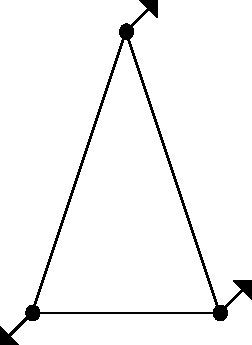
\includegraphics[width=\linewidth]{images/tri_collocated.pdf}
             \label{fig:tricollo}
         \end{subfigure}
         \hspace{0.1\linewidth}
         \begin{subfigure}[b]{0.15\linewidth}
             \centering
             \includegraphics[width=\linewidth]{images/tri_staggered.pdf}
             \label{fig:tristagg}
         \end{subfigure}
         \label{fig:celulas}
    \end{figure}
\end{frame}


%----------------------------------------------------------------------------------------

\begin{frame}
\frametitle{Simulação de fluidos}
    \begin{block}{Diferenças finitas}
        \begin{itemize}
            \item Realiza o cálculo de operadores diferenciais
            \item Baseado na série de Taylor
            \item Dependente da estrutura da malha
            \item Três tipos: Progressiva, regressiva e central.
        \end{itemize}
    \end{block}
\end{frame}

%----------------------------------------------------------------------------------------

\begin{frame}
\frametitle{Simulação de fluidos}
    \begin{block}{\emph{Pipeline} de simulação do \emph{Stable Fluids}}
        \begin{itemize}
            \item Adição de forças externas 
            \item Advecção
            \item Projeção de pressão
        \end{itemize}
    \end{block}
    \begin{figure}
        \centering
        \includegraphics[width=0.9\linewidth]{images/diag0.pdf}
        \caption{Pipeline de simulação}
        \label{fig:malha_estruturada+}
    \end{figure}
\end{frame}

%----------------------------------------------------------------------------------------

\begin{frame}{Stam 2D implementado}
    \movie[width=3cm,height=2cm,poster]{}{images/stam2d.mp4}
\end{frame}{}
%----------------------------------------------------------------------------------------



\begin{frame}
\section{RBF-FD}
\frametitle{RBF-FD}
    \begin{block}{\emph{RBF Liquids: An Adaptive PIC Solver Using RBF-FD} (Nakanishi, 2020)}
        \begin{itemize}
            \item Quadtree e Octree
            \item Adaptativa
            \item Não-conforme
            \item RBF-FD
            \item Não impõe a condição de contorno Neumann em fronteiras arbitrárias
        \end{itemize}
    \end{block}
    \begin{figure}
        \centering
        \includegraphics[width=0.8\linewidth]{images/naka.png}
        \label{fig:my_label}
    \end{figure}
\end{frame}

%----------------------------------------------------------------------------------------

\begin{frame}
\frametitle{RBF-FD}
    \begin{block}{RBF}
        Uma RBF é uma função radialmente simétrica entre o centro $x_k$ e o ponto avaliado $x$. Representada por $\Phi_k(\mathbf{x}) = \phi(||\mathbf{x}-\mathbf{x}_k||)$, onde $\phi(r)$ representa uma função escalar $[0, \infty)$ e $||\cdot||$ denota a norma euclidiana. Existem várias escolhas para $\phi$, uma é a \emph{spline} poliharmônica $\phi(r) = r^s$, com s = 1, 3, 5,...
    \end{block}

    \begin{block}{Interpolador RBF}
        Aproximação de diferenças finitas por meio do uso de RBFs. Seja uma nuvem de pontos, $\{x_k\}_{k=1}^N$, os valores das funções $y_k=y(x_k)\in\mathbb{R}$, queremos acha um interpolador $S_y: \Omega \xrightarrow{} \mathbb{R}$, tal que:
        \begin{equation}
            S_y(x_i)=y_i\,\text{,   }\forall i = 1, ..., N\,.
        \end{equation}
    \end{block}
\end{frame}

%----------------------------------------------------------------------------------------

\begin{frame}
\frametitle{RBF-FD}
    \begin{block}{Forma geral}
        A forma generalizada de um interpolador RBF é dada por:
        \begin{equation}
            S_y(x) = \sum_{k=1}^N \omega_k \phi(||x-x_k||) + \sum^M_{j=1}\gamma_jP_j(x)\,\text{, onde}\sum_{k=1}^N\omega_k P_j(x_k) = 0\,\text{,   }\forall 1,...,M.
            \label{eq:rbf0}
        \end{equation}
        
    \end{block}

    \begin{block}{Aproximando um operador diferencial}
        Seja $\mathcal{L}$ o operador diferencial que queremos aproximar, e $\mathcal{X}_i$ a vizinhança composta por uma nuvem de pontos $\{x_k\}_{k=1}^N$. Para uma dada posição $x_i$, queremos aproximar $\mathcal{L}y$ avaliado no ponto central $x_i$ como uma combinação linear dos valores das funções $\{y_k\}_{k=1}^N$, tal que:

        \begin{equation}
            \mathcal{L}y = \sum_{k=1}^N\omega_k^\mathcal{L}y_k\,.
        \end{equation}
        %
        
    \end{block}
\end{frame}

%----------------------------------------------------------------------------------------

\begin{frame}

\frametitle{RBF-FD}
    \begin{block}{Cálculo dos pesos}
        Os pesos $\omega$ são obtidos resolvendo o seguinte sistema:
        
        \begin{equation}
            \left[ 
                \begin{array}{cc}
                    \mathbf{A}
                     & 
                    \mathbf{P}\\
                   
                   \mathbf{P}^T& 
                   \mathbf{O}\\
                \end{array} 
            \right]
            \left[ 
                \begin{array}{c}
                    \mathbf{\omega}^\mathcal{L}\\
                   \mathbf{\gamma}
                \end{array} 
            \right]
            =
            \left[ 
                \begin{array}{c}
                    \mathbf{\mathcal{L}\phi}\\
                    \mathbf{\mathcal{L}\mathbf{P}}
                \end{array} 
            \right]\,,
            \label{eq:pesos_rbf}
        \end{equation}
        \begin{itemize}
            \item $\mathbf{A}$ é uma matriz de ordem $N$ com $\mathbf{A}_{ij} = \phi(||x_i-x_j)||$
            \item $\mathbf{P}$ é uma matriz de ordem $N \times M$ e $\mathbf{P}_{ij}=P_j(x_i)$
            \item $\mathbf{O}$ é uma matriz nula de ordem $M$
            \item $\mathbf{\omega}^\mathcal{L}=[\omega_1^\mathcal{L},...\omega_N^\mathcal{L}]^{\top}$
            \item $\mathbf{\gamma}=[\gamma_1,...\gamma_M]^{\top}$
        \end{itemize}
    \end{block}
\end{frame}{}

%----------------------------------------------------------------------------------------

\begin{frame}{RBF-FD}
    \begin{block}{Matriz de cálculo dos pesos}
        Dado uma vizinhança $\mathcal{X}_i$ composta por uma nuvem de pontos $\{x_k\}_{k=1}^N$. Com s = 5 e ordem do polinômio = 2. Com $\Phi_k(\mathbf{x}) = \phi(||\mathbf{x}-\mathbf{x}_k||)$
        \[
        \mathbf{A} = \begin{bmatrix} 
            \Phi_1(x_1) & \dots  & \Phi_N(x_1)\\
            \vdots & \ddots & \vdots\\
            \Phi_1(x_N) & \dots  & \Phi_N(x_N)
            \end{bmatrix}
        \]
        \[
        \mathbf{P} = \begin{bmatrix} 
            1 & x1  & y1 & x1y1 & x1^2 & y1^2\\
            \vdots & \vdots & \vdots& \vdots& \vdots& \vdots\\
            1 & xN  & yN & xNyN & xN^2 & yN^2    
            \end{bmatrix}
        \]
        \[
        \mathbf{\mathbf{\mathcal{L}\phi}} = \begin{bmatrix} 
            \mathbf{\mathcal{L}\Phi_k(x_1)}\\
            \vdots\\
            \mathbf{\mathcal{L}\Phi_k(x_N)}   
            \end{bmatrix}
        \]        
    \end{block}{}    
\end{frame}
%----------------------------------------------------------------------------------------

\begin{frame}{RBF-FD}
    \begin{block}{Matriz de cálculo dos pesos}
        Dado uma vizinhança $\mathcal{X}_i$ composta por uma nuvem de pontos $\{x_k\}_{k=1}^N$. Com s = 5 e ordem do polinômio = 2. Com $\Phi_k(\mathbf{x}) = \phi(||\mathbf{x}-\mathbf{x}_k||)$.
        Caso $\mathbf{\mathcal{L}}$ seja o laplaciano:
        \[
        \mathbf{\mathbf{\mathcal{L}P}} = \begin{bmatrix} 
            0\\
            0\\
            0\\
            0\\
            2\\
            2
            \end{bmatrix}
        \]
        
    \end{block}{}    
\end{frame}

%----------------------------------------------------------------------------------------

\begin{frame}

\frametitle{RBF-FD}
    \begin{block}{Calculando os operadores diferenciais necessários}
        Calculamos os pesos RBF para o laplaciano, derivada parcial em x e derivada parcial em y. Com isso conseguimos calcular grandiente, divergente, laplaciano e impor Neumann na fronteira.
    \end{block}
    \begin{block}{Impondo Neumann na fronteira}
        A condição de contorno de Neumann homogênea é dada por, sendo $p$ o campo escalar:
        \begin{equation}
            \frac{\partial p}{\partial\mathbf{n}} = \mathbf{n}\cdot\nabla p = 0
        \end{equation}{}
        Quando o nó central($p_k$) está na fronteira, fazemos o cálculo dos pesos que vão para a matriz de Poisson da seguinte maneira: 
        \begin{equation}
            n_x\sum_k\omega_k^xp_k + n_y\sum_k\omega_k^yp_k = \sum_k (n_x\omega_k^x + n_y\omega_k^y)p_k
        \end{equation}{}
    \end{block}
    
\end{frame}{}


%----------------------------------------------------------------------------------------

\begin{frame}

\frametitle{RBF-FD}
    \begin{block}{Cálculo da vizinhança}
        Utilizamos o K-anel do vértice para obter a vizinhança
    \end{block}
    \begin{figure}
        \centering
        \includegraphics[width=0.5\linewidth]{images/nring_int.png}
        \label{fig:my_label}
        \caption{2-anel no interior}
    \end{figure}{}
\end{frame}{}

%----------------------------------------------------------------------------------------
\begin{frame}
\frametitle{Simulação de fluidos: Passo a Passo}
    \begin{block}{\emph{Pipeline} de simulação do \emph{Stable Fluids}}
        \begin{itemize}
            \item Adição de forças externas: Integração de Euler
            \item Advecção 
            \item Projeção de pressão
        \end{itemize}
    \end{block}
    \begin{figure}
        \centering
        \includegraphics[width=0.9\linewidth]{images/diag1.pdf}
        \caption{Pipeline de simulação}
        \label{fig:malha_estruturada+}
    \end{figure}
\end{frame}

%----------------------------------------------------------------------------------------

\begin{frame}
\frametitle{Simulação de fluidos: Passo a Passo}
    \begin{block}{\emph{Pipeline} de simulação do \emph{Stable Fluids}}
        \begin{itemize}
            \item Adição de forças externas
            \item Advecção: Esquema semi-lagrangiano
            \item Projeção de pressão 
        \end{itemize}
    \end{block}
    \begin{figure}
        \centering
        \includegraphics[width=0.9\linewidth]{images/diag2.pdf}
        \caption{Pipeline de simulação}
        \label{fig:malha_estruturada+}
    \end{figure}
\end{frame}

%----------------------------------------------------------------------------------------

\begin{frame}
\frametitle{Simulação de fluidos: Passo a Passo}
    \begin{block}{\emph{Pipeline} de simulação do \emph{Stable Fluids}}
        \begin{itemize}
            \item Adição de forças externas
            \item Advecção: Esquema semi-lagrangiano
            \item Projeção de pressão 
        \end{itemize}
    \end{block}
    \begin{figure}
        \centering
        \includegraphics[width=0.35\linewidth]{images/tri_backtracking.pdf}
        \caption{Esquema de backtracking}
        \label{fig:malha_estruturada+}
    \end{figure}
\end{frame}

%----------------------------------------------------------------------------------------

\begin{frame}
\frametitle{Simulação de fluidos: Passo a Passo}
    \begin{block}{\emph{Pipeline} de simulação do \emph{Stable Fluids}}
        \begin{itemize}
            \item Adição de forças externas
            \item Advecção
            \item Projeção de pressão: $\nabla^2p=\nabla\cdot\mathbf{u}$, $\mathbf{u} =  \mathbf{u} - \nabla p$
        \end{itemize}
    \end{block}
    \begin{figure}
        \centering
        \includegraphics[width=0.9\linewidth]{images/diag3.pdf}
        \caption{Pipeline de simulação}
        \label{fig:malha_estruturada+}
    \end{figure}
\end{frame}


%----------------------------------------------------------------------------------------

\begin{frame}{Simulação de fluidos: Passo a Passo}
    \begin{block}{Matriz de Poisson}
        Dado a seguinte malha:
        \begin{figure}
            \centering
            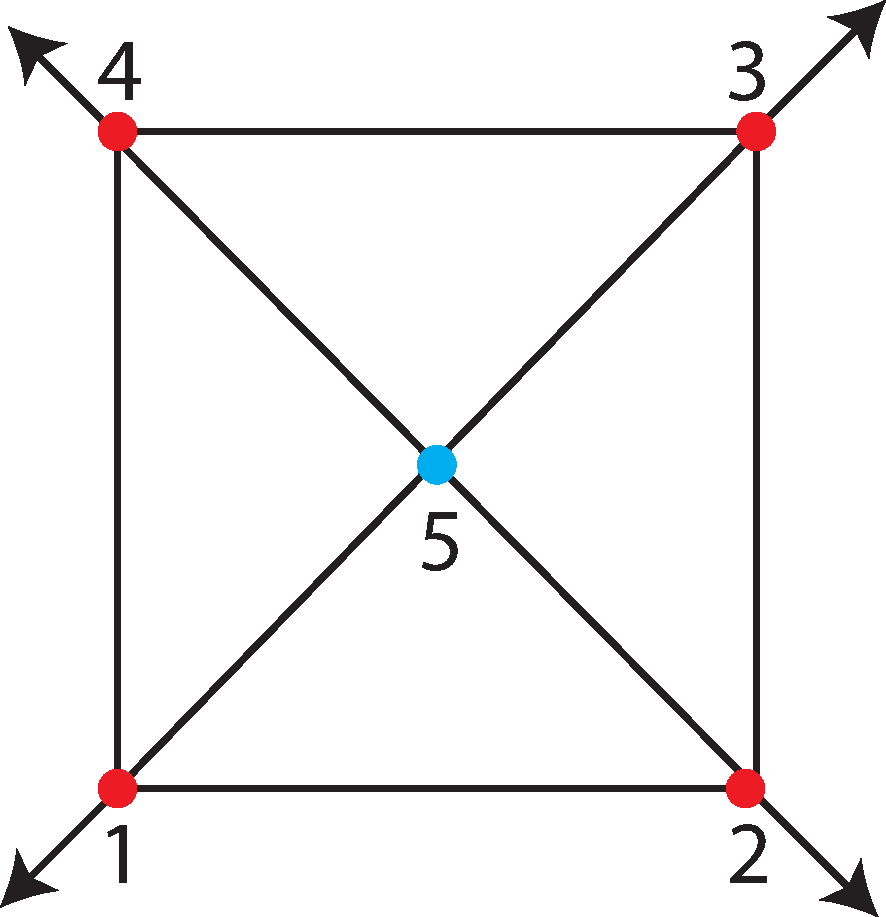
\includegraphics[width=0.4\linewidth]{images/mesh-simple.pdf}
            \label{fig:my_label}
        \end{figure}{}
    \end{block}{}    
\end{frame}

%----------------------------------------------------------------------------------------

\begin{frame}{Simulação de fluidos: Passo a Passo}
    \begin{block}{Matriz de Poisson}
        Com os pesos calculados, e usando o 1-anel como vizinhança, podemos montar a matriz para resolver a equação de poisson da seguinte maneira.
        \begin{figure}
            \centering
            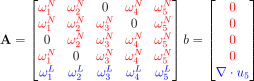
\includegraphics[width=0.8\linewidth]{images/CodeCogsEqn.pdf}
            \caption{Matriz de poisson com imposição de Neumann na fronteira}
            \label{fig:my_label}
        \end{figure}{}
        Com $\omega_k^N = n_x\omega_k^x + n_y\omega_k^y$
        
    \end{block}{}    
\end{frame}
%----------------------------------------------------------------------------------------

\begin{frame}
\section{Proposta}
\frametitle{Proposta}
    \begin{block}{Proposta}
        Utilizar os operadores diferenciais calculados por meio de RBF-FD em uma malha não estruturada para realizar a simulação de fumaça utilizando o pipeline apresentado.
    \end{block}
    \begin{table}[H]
    \centering
    \caption{Cronograma}
    \begin{tabular}{cccccc}
    \hline
                          & 2021/1 & 2021/2 & 2022/1 & 2022/2 & 2023/1\\ \hline
    Revisão Bibliográfica & $\times$      & $\times$      & $\times$      & $\times$      &$\times$\\
    Grade regular 2D      & $\times$      & $\times$      &        &       & \\
    Grade não-estruturada &        &        & $\times$      & $\times$   &   \\
    Pipeline com RBF-FD      &        &        &        & $\times$   & $\times$ \\
    Domínios arbitrários      &        &        &        & $\times$   & $\times$ \\\hline
    \end{tabular}
    \end{table}
\end{frame}

%----------------------------------------------------------------------------------------

\begin{frame}
\section{Resultados parciais}
\frametitle{Resultados parciais}
    Foram realizados teste com funções analíticas e malhas triangulares com domínios AABB fazendo o uso da normal para impor Neumann. Para cálculo dos pesos RBF, utilizamos s=5, d=2, k=2. $\Omega = [0,\pi]^2$
    \begin{block}{Malha não estruturada}
        \begin{figure}
            \centering
            \includegraphics[width=0.5\linewidth]{images/mesh.pdf}
            \caption{Malha 16x16}
            \label{fig:my_label}
        \end{figure}
    \end{block}
\end{frame}

%----------------------------------------------------------------------------------------

\begin{frame}
\frametitle{Resultados parciais}
    \begin{block}{Equação de Poisson}
        $\nabla^2f(x,y) = -2\cos(x)\cos(y)$ \\
        Solução : $f(x,y) = \cos(x)\cos(y) - 1$. 
        $\frac{\partial f}{\partial\mathbf{n}}=0,\, \forall (x,y) \in \partial\Omega$
        \begin{figure}
            \centering
            \includegraphics[width=0.6\linewidth]{images/poisson_error.pdf}
            \caption{Erro da equação de Poisson em malha 16x16}
            \label{fig:my_label}
        \end{figure}
    \end{block}
\end{frame}

%----------------------------------------------------------------------------------------

\begin{frame}
\frametitle{Resultados parciais}
    \begin{block}{Divergente}
        $F(x,y) = (-2\cos(x)\cos(y), -2\cos(x)\cos(y))$\\
        Solução: $\nabla\cdot f(x,y) = 2\sin(x+y)$
        \begin{figure}
            \centering
            \includegraphics[width=0.7\linewidth]{images/div_error.pdf}
            \caption{Erro do divergente em malha 16x16}
            \label{fig:my_label}
        \end{figure}
    \end{block}
\end{frame}

%----------------------------------------------------------------------------------------

\begin{frame}
\frametitle{Resultados parciais}
    \begin{block}{Gradiente}
        $f(x,y) = -2\cos(x)\cos(y)$\\
        Solução: $\nabla F(x,y) = (2cos(y)sin(x), 2cos(x)sin(y))$
        \begin{figure}
            \centering
            \includegraphics[width=0.7\linewidth]{images/grad_error.pdf}
            \caption{Erro do gradiente em malha 16x16}
            \label{fig:my_label}
        \end{figure}
    \end{block}
\end{frame}

%----------------------------------------------------------------------------------------

\begin{frame}
\section{Resultados esperados}
\frametitle{Resultados esperados}
    \begin{block}{Resultados esperados}
        Implementação da simulação de fumaça 2D/3D em domínios arbitrários.
    \end{block}
\end{frame}

%----------------------------------------------------------------------------------------

\begin{frame}
\frametitle{Conclusão}
\centering 
    \Huge{Obrigado!}
\end{frame}


%------------------------------------------------

% \begin{frame}
% \frametitle{Bullet Points}
% \begin{itemize}
% \item Lorem ipsum dolor sit amet, consectetur adipiscing elit
% \item Aliquam blandit faucibus nisi, sit amet dapibus enim tempus eu
% \item Nulla commodo, erat quis gravida posuere, elit lacus lobortis est, quis porttitor odio mauris at libero
% \item Nam cursus est eget velit posuere pellentesque
% \item Vestibulum faucibus velit a augue condimentum quis convallis nulla gravida
% \end{itemize}
% \end{frame}

% %------------------------------------------------

% \begin{frame}
% \frametitle{Blocks of Highlighted Text}
% \begin{block}{Block 1}
% Lorem ipsum dolor sit amet, consectetur adipiscing elit. Integer lectus nisl, ultricies in feugiat rutrum, porttitor sit amet augue. Aliquam ut tortor mauris. Sed volutpat ante purus, quis accumsan dolor.
% \end{block}

% \begin{block}{Block 2}
% Pellentesque sed tellus purus. Class aptent taciti sociosqu ad litora torquent per conubia nostra, per inceptos himenaeos. Vestibulum quis magna at risus dictum tempor eu vitae velit.
% \end{block}

% \begin{block}{Block 3}
% Suspendisse tincidunt sagittis gravida. Curabitur condimentum, enim sed venenatis rutrum, ipsum neque consectetur orci, sed blandit justo nisi ac lacus.
% \end{block}
% \end{frame}

% %------------------------------------------------

% \begin{frame}
% \frametitle{Multiple Columns}
% \begin{columns}[c] % The "c" option specifies centered vertical alignment while the "t" option is used for top vertical alignment

% \column{.45\textwidth} % Left column and width
% \textbf{Heading}
% \begin{enumerate}
% \item Statement
% \item Explanation
% \item Example
% \end{enumerate}

% \column{.5\textwidth} % Right column and width
% Lorem ipsum dolor sit amet, consectetur adipiscing elit. Integer lectus nisl, ultricies in feugiat rutrum, porttitor sit amet augue. Aliquam ut tortor mauris. Sed volutpat ante purus, quis accumsan dolor.

% \end{columns}
% \end{frame}

% %------------------------------------------------
% \section{Second Section}
% %------------------------------------------------

% \begin{frame}
% \frametitle{Table}
% \begin{table}
% \begin{tabular}{l l l}
% \toprule
% \textbf{Treatments} & \textbf{Response 1} & \textbf{Response 2}\\
% \midrule
% Treatment 1 & 0.0003262 & 0.562 \\
% Treatment 2 & 0.0015681 & 0.910 \\
% Treatment 3 & 0.0009271 & 0.296 \\
% \bottomrule
% \end{tabular}
% \caption{Table caption}
% \end{table}
% \end{frame}

% %------------------------------------------------

% \begin{frame}
% \frametitle{Theorem}
% \begin{theorem}[Mass--energy equivalence]
% $E = mc^2$
% \end{theorem}
% \end{frame}

% %------------------------------------------------

% \begin{frame}[fragile] % Need to use the fragile option when verbatim is used in the slide
% \frametitle{Verbatim}
% \begin{example}[Theorem Slide Code]
% \begin{verbatim}
% \begin{frame}
% \frametitle{Theorem}
% \begin{theorem}[Mass--energy equivalence]
% $E = mc^2$
% \end{theorem}
% \end{frame}\end{verbatim}
% \end{example}
% \end{frame}

% %------------------------------------------------

% \begin{frame}
% \frametitle{Figure}
% Uncomment the code on this slide to include your own image from the same directory as the template .TeX file.
% \begin{figure}
% \includegraphics[width=0.8\linewidth]{test.png}
% \end{figure}
% \end{frame}

% %------------------------------------------------

% \begin{frame}[fragile] % Need to use the fragile option when verbatim is used in the slide
% \frametitle{Citation}
% An example of the \verb|\cite| command to cite within the presentation:\\~

% This statement requires citation \cite{p1}.
% \end{frame}

% %------------------------------------------------



% %------------------------------------------------

% \begin{frame}
% \Huge{\centerline{The End}}
% \end{frame}

%----------------------------------------------------------------------------------------

\end{document} 